\documentclass{beamer}


\usepackage{tikz}
\usetikzlibrary{positioning,shapes.geometric}

\usetheme{Warsaw}

\title[ On the affect of ``attempting to lose weight'' on sleep ]{Project Presentation}

\author{Alex Luedtke, Lucia Petito, Steven Pollack}
\institute{PHC252D}
\date{}

\begin{document}
\maketitle 
\begin{frame}
 \frametitle{Outline} % need causal roadmap.
  \begin{itemize}
    \item Background
    \item Specify SCM (and DAG)
    \item Specify counterfactuals and target causal quantity
    \item Introduce data and commit to a statistical model
    \item Discuss identifiability and estimand
    \item Get our hands dirty (estimation procedures)
    \item Results
    \item Interpretation
  \end{itemize}
\end{frame}

\begin{frame}
 \frametitle{Background}
 We know that sleep affects weight, but does trying to lose weight affect sleep?
 \begin{itemize}
  \item We used National Health and Nutrition Examination Survey (NHANES) data -- from the National Center for Health Statistics (NCHS) -- a multistage survey of U.S. population
    \begin{itemize}
      \item Stage 1: Counties
      \item Stage 2: Segments
      \item Stage 3: Households
      \item Stage 4: Individuals
    \end{itemize}
  \item Survey aims to study wide range of topics such as Cardiovascular disease, Obesity, Physical fitness and physical functioning, Reproductive history and sexual behavior, etc.
  \end{itemize}
\end{frame}

\begin{frame}
  \frametitle{Background (Cont'd)}
  Notes about NHANES data:
  \begin{itemize}
 \item Individuals were subjected to interviews as well as physical examinations.
  \begin{itemize}
    \item categorical as well as numerical data
    \item some questions had a lot of valid responses, but made positivity questionable.
    \item No shortage of missing data (either ``I don't know'''s or unanswered questions).
  \end{itemize}
 \item The sample for the survey is selected to represent the U.S. population of all ages. To produce reliable statistics, NHANES over-samples persons 60 and older, African Americans, and Hispanics.
 \end{itemize}
\end{frame}

\begin{frame}
\frametitle{SCM and DAG}
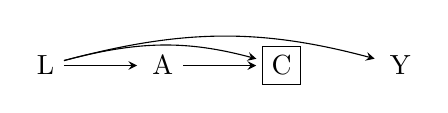
\begin{tikzpicture}[%
->,
shorten >=2pt,
>=stealth,
node distance=1cm,
pil/.style={
->,
thick,
shorten =2pt,}
]
\node (2) {A};
\node[left =of 2] (1) {L};
\node[rectangle,draw] [right=of 2] (4) {C};
\node[right= of 4] (3) {Y};
\draw[->] (1.east) --(2.west);
\draw[->] (2.east) -- (4.west);
\draw[->] (1) to [out=15,in=165] (3);
\draw[->] (1) to [out=15,in=165] (4);
\end{tikzpicture}
\end{frame}

\begin{frame}
\frametitle{$W$: Baseline Covariates}
   \begin{itemize}
   \item Gender \\
   \item Age in months (300-959 months, 25-79 years) \\
   \item Race/Ethnicity (Mexican American, Other Hispanic, Non-Hispanic White, Non-Hispanic Black, Other) \\
   \item Education Level (less than high school, high school/GED, some college, college and above) \\
   \item Marital Status (never married, married/living with partner, divorced/separated) \\
   \item Annual Household Income (less than or greater than \$20k) \\
   \item Body Mass Index (continuous from 15-50) \\
   \item DELETE ME ****
  \end{itemize}

\end{frame}

\begin{frame}
 \frametitle{$A$: Exposure Variable}
  \begin{itemize}
    \item 
  \end{itemize}

\end{frame}

\begin{frame}
 \frametitle{$Y$: Response Variable}
  \begin{itemize}
    \item 
  \end{itemize}

\end{frame}

\begin{frame}
 \frametitle{Specify  SCM (and DAG)}
  \begin{itemize}
    \item 
  \end{itemize}

\end{frame}

\end{document}